\documentclass[10pt]{article}
\usepackage{mathtools}
\usepackage{amsmath}
\usepackage{tabularx}
\usepackage{graphicx}
\usepackage{flexisym}
\usepackage{listings}
\usepackage{xcolor}
\usepackage{hyperref}
\usepackage{amsthm}
\usepackage{subcaption}
\newtheorem*{theorem}{Theorem}
\begin{document}
\setlength\parindent{1pt}
\title{Building a model for the solar system using ordinary differential equations}
\author{Andrei Kukharenka and Anna Gribkovskaya \\  
FYS 4150 
}

\maketitle
\begin{abstract}
In this project we built a model for the solar system using Newtonian's law of gravity. This lead to a system of ordinary differential equations (ODE) to be solved numerically. Verlet method shows good convergence while Euler's method is not stable. Using Verlet solver we showed that solar system is stable. Also the influence of the Jupiter on the Earth motion was studied. Finally we calculated procession of Mercury's perihelion by correcting a force to conform it with general relativity. Results are in good agreement with astronomical data. 
\end{abstract}
\clearpage 


\section{Introduction}
Simulations are extremely important tool in nowadays science. It provides us a deeper understanding of nature and  better insight into the processes taking place in a complicated systems. It is also very useful for presenting and analyzing the results.\\
In this project our goal was to simulate the solar system using Newtonian law of gravity. We end up with a system of ODEs, which can be solved numerically. We considered finite difference methods, namely velocity Verlet and Euler. In our model of the solar system all celestial bodies have constant masses and all general relativistic effects are neglected except the case we study precession of the Mercury's perihelion. We tested two numerical methods mentioned above and chose one based on numerical precision, stability and convergence rate. We also studied the special case for three bodies to investigate Jupiter's influence on the Earth orbit. All deformation effects which may be caused by gravity forces were neglected. Additionally we tested our simulation to provide observed precession of Mercury's perihelion considering general relativity correction to the Newtonian gravitational force.\\
It was shown that object oriented programming approach is very useful for such simulations. We created a special class for celestial bodies in order to store information we need to use and update during the simulation. \\
The report has the following structure:\\*
In the part \ref{Part1}  we discuss the problem and make assumptions to the model of the solar system, then we present Verlet and Euler methods for solving ODEs and discuss their precision (part \ref{Numerical methods}). Those who are already familiar with those methods can safely skip this part and go directly to the results and discussion part \ref{results}  where we present simulated results. In conclusion \ref{conc} we made a brief overview of obtained results and discuss possibilities for further research. 

 

\newpage
\section{Problem formulation and mathematical method}\label{Part1}
In this part we present a mathematical description of investigated problem as well as derivation and discussion of numerical methods to be used for simulations.  Model of the Solar system is based on Newtonian gravity law. 

\subsection{The gravity and laws of motion}
To provide an appropriate description of the planetary motion we need to consider the only force in the solar system  -- gravity. Newton's law of gravitation stands that two bodies with masses $M_1$ abd $M_2$ are attracted to each other with a force given by:
\[
F_G=\frac{GM_{1}M_{2}}{r^2},
\]
where $r$ is the distance between objects and $G$ is the gravitational constant.
Applying  Newton's second law of motion to our problem we get the following equations:
\[
\frac{d^2x}{dt^2}=\frac{F_{G,x}}{M_{\mathrm{Earth}}},
\]
, 
\[
\frac{d^2y}{dt^2}=\frac{F_{G,y}}{M_{\mathrm{Earth}}},
\]
and
\[
\frac{d^2z}{dt^2}=\frac{F_{G,z}}{M_{\mathrm{Earth}}},
\]
where $F_{G,x}$, $F_{G,y}$ and $F_{G,z}$ are the $x$, $y$ and $z$ components of the gravitational force, $M_{\mathrm{Earth}}$ is the mass of the Earth.
Lets assume that mass of the Sun is much larger then mass of the Earth and that orbit of the Earth is circular. In this case Cartesian coordinates of Earth can be easily rewritten from spherical coordinates (radius $r$, inclination $\theta$ and azimuth $\varphi$):

\[
x=r cos\varphi sin\theta,
\]
\[
y=r sin\varphi\cos\theta,
\]
and
\[
r=\sqrt{x^2+y^2+z^2},
\]
It's obvious that:
\[
{F_{G,x}}=-G\frac{M_{\mathrm{E}}M_{\odot}}{r^2}cos\varphi sin\theta
\]
Where $M_{\mathrm{E}}$ and $M_{\odot}$ are masses of the Earth and the Sun correspondingly. By multiplying and dividing right hand side of the last equation by $x$ we get new equation for the $x$-component of the gravitational force between the Sun and the Earth:

\begin{equation}\label{eq:force_motion}
F_{G,x}=-Gx\frac{M_{\mathrm{E}}M_{\odot}}{r^3},
\end{equation}
Similarly one can obtain equations for remaining force components:
\[
{F_{G,y}}=-Gy\frac{M_{\mathrm{E}}M_{\odot}}{r^3}
\]
and
\[
{F_{G,z}}=-Gz\frac{M_{\mathrm{E}}M_{\odot}}{r^3}.
\]
Now let us take into considerations values of astronomical constants. If one uses SI units the mass of the Sun is $M_{\odot}=2\times 10^{30}$ kg, the mass of Earth is $M_{\mathrm{E}}=6\times 10^{24}$ kg, gravitational constant $G=6.67408 \times 10^{-11}$ $m^3 \cdot kg^{-1} \cdot s^{-2}$ and distance between the Earth and the Sun is $r=1.5 \times 10^{11}$ m. If all mentioned values will be used in SI units during numerical calculations we can easily get loss of numerical precision due to round-off errors. Considering order of magnitude of mentioned constants we presume that the best units to use in this case are astronomical units. Clarifying and summarizing just mentioned
above we will use $1AU=1.5 \times 10^{11}$ m as lengths units, $Earth's\ years$ as time units and all masses will be expressed in terms of the Sun masses $M_{\odot}$. Careful reader may notice that we didn't tell anything about the gravitational constant. We are going to derive it using an assumption of circular orbit of the Earth.
Considering that in our model of the solar system planets are moving uniformly depicting a circle we can write:
\[
\frac{M_{\mathrm{E}}v^2}{r}=G\frac{M_{\mathrm{E}}M_{\odot}}{r^2},
\]
where $v$ is velocity of the Earth.
The latter equation can be used to show:
\begin{equation}\label{eq:getridofg}
GM_{\odot} = 4\pi^2 \Bigg[ \frac{AU^3}{year^2}\Bigg]
\end{equation}
Using \ref{eq:getridofg} we can rewrite equation of motion and get rid of gravitational constant:

\begin{equation}\label{eq:motion}
\begin{aligned}
\frac{dv_x}{dt}=-4\pi^2\frac{x}{r^3} \Bigg[ \frac{AU^3}{year^2}\Bigg]\ \& \ \frac{dx}{dt} = v_x,\\
\frac{dv_y}{dt}=-4\pi^2\frac{y}{r^3} \Bigg[ \frac{AU^3}{year^2}\Bigg]\ \& \ \frac{dy}{dt} = v_y, \\
\frac{dv_z}{dt}=-4\pi^2\frac{z}{r^3} \Bigg[ \frac{AU^3}{year^2}\Bigg]\ \& \ \frac{dz}{dt} = v_z.
\end{aligned}
\end{equation}

\subsection{The three-body problem}
In previous section we obtained equations of motion for two bodies in gravitational field. Hoverer it is experimentally proven that our solar system has number of planets that is more than one. Let us try to scale discussed problem to three bodies.
We add to the system discussed above one more celestial body for example the Jupiter. Now each body interacts with each other.
Equation \ref{eq:force_motion} for interaction between the Earth and the Jupiter can be rewritten then as:
\begin{equation}\label{eq:motion_3body}
F_{G,x}^{\mathrm{EJ}}=-G(x_{\mathrm{E}}-x_{\mathrm{J}})\frac{M_{\mathrm{E}}M_{\mathrm{J}}}{r^3_{\mathrm{EJ}}},
\end{equation}
with 
\[
r_{\mathrm{EJ}}=\sqrt{(x_{\mathrm{E}}-x_{\mathrm{J}})+(y_{\mathrm{E}}-y_{\mathrm{J}})+(z_{\mathrm{E}}-z_{\mathrm{J}})},
\]
where $x_{\mathrm{J}}$, $y_{\mathrm{J}}$, $z_{\mathrm{J}}$ are Cartesian coordinates of the Jupiter with the Sun in the origin, $M_{\mathrm{E}}$ is mass of the Jupiter.
Taking into account interaction with the Sun we can rewrite \ref{eq:motion} for three-body problem:

\begin{equation}\label{eq:motion-3-earth}
\begin{aligned}
\frac{dv_x^{\mathrm{E}}}{dt}=-4\pi^2\frac{x_{\mathrm{E}}}{r^3} \Bigg[ \frac{AU^3}{year^2}\Bigg] - 4\pi^2\frac{M_{\mathrm{J}}}{M_{\odot}}\frac{x_{\mathrm{E}}-x_{\mathrm{J}}}{r_{\mathrm{EJ}}^3} \Bigg[ \frac{AU^3}{year^2}\Bigg]\ \& \ \frac{dx_{\mathrm{E}}}{dt} = v_x^{\mathrm{E}},\\
\frac{dv_y^{\mathrm{E}}}{dt}=-4\pi^2\frac{y_{\mathrm{E}}}{r^3} \Bigg[ \frac{AU^3}{year^2}\Bigg] - 4\pi^2\frac{M_{\mathrm{J}}}{M_{\odot}}\frac{y_{\mathrm{E}}-y_{\mathrm{J}}}{r_{\mathrm{EJ}}^3} \Bigg[ \frac{AU^3}{year^2}\Bigg],\ \& \ \frac{dy_{\mathrm{E}}}{dt} = v_y^{\mathrm{E}},\\
\frac{dv_z^{\mathrm{E}}}{dt}=-4\pi^2\frac{z_{\mathrm{E}}}{r^3} \Bigg[ \frac{AU^3}{year^2}\Bigg] -4\pi^2\frac{M_{\mathrm{J}}}{M_{\odot}}\frac{z_{\mathrm{E}}-z_{\mathrm{J}}}{r_{\mathrm{EJ}}^3} \Bigg[ \frac{AU^3}{year^2}\Bigg]\ \& \ \frac{dz_{\mathrm{E}}}{dt} = v_z^{\mathrm{E}}.
\end{aligned}
\end{equation}  
Similarly one can easy get equations for the Jupiter:
\begin{equation}\label{eq:motion-3-jupiter}
\begin{aligned}
\frac{dv_x^{\mathrm{J}}}{dt}=-4\pi^2\frac{x_{\mathrm{J}}}{r_{\mathrm{SJ}}^3} \Bigg[ \frac{AU^3}{year^2}\Bigg] + 4\pi^2\frac{M_{\mathrm{J}}}{M_{\odot}}\frac{x_{\mathrm{E}}-x_{\mathrm{J}}}{r_{\mathrm{EJ}}^3} \Bigg[ \frac{AU^3}{year^2}\Bigg]\ \& \ \frac{dx_{\mathrm{J}}}{dt} = v_x^{\mathrm{J}},\\
\frac{dv_y^{\mathrm{J}}}{dt}=-4\pi^2\frac{y_{\mathrm{J}}}{r_{\mathrm{SJ}}^3} \Bigg[ \frac{AU^3}{year^2}\Bigg] + 4\pi^2\frac{M_{\mathrm{J}}}{M_{\odot}}\frac{y_{\mathrm{E}}-y_{\mathrm{J}}}{r_{\mathrm{EJ}}^3} \Bigg[ \frac{AU^3}{year^2}\Bigg]\ \& \ \frac{dy_{\mathrm{J}}}{dt} = v_y^{\mathrm{J}}, \\
\frac{dv_z^{\mathrm{J}}}{dt}=-4\pi^2\frac{z_{\mathrm{J}}}{r_{\mathrm{SJ}}^3} \Bigg[ \frac{AU^3}{year^2}\Bigg] + 4\pi^2\frac{M_{\mathrm{J}}}{M_{\odot}}\frac{z_{\mathrm{E}}-z_{\mathrm{J}}}{r_{\mathrm{EJ}}^3} \Bigg[ \frac{AU^3}{year^2}\Bigg]\ \& \ \frac{dz_{\mathrm{J}}}{dt} = v_z^{\mathrm{J}}.
\end{aligned}
\end{equation}  

\subsection{Numerical methods}\label{Numerical methods}

We managed to rewrite our second order differential equations as coupled first order differential equations \ref{eq:motion} and \ref{eq:motion-3-jupiter} which can be solved by different numerical methods. In this project we focus only on finite difference methods. We consider Euler and velocity Verlet methods bellow, however there are many others for example family of Runge-Kutta methods.
Here we start with discussion of Euler's method which is rather simple but gives a good feeling of all finate difference methods for solving ODEs.\\
\subsubsection{Forward Euler's method}

We have the ODE of the form: 
\[
\frac{dy}{dt}=f(t,y),
\] 
Assume we have initial conditions $y_0 = y(t_0)$. We discretize a time domain and use the Taylor expansion for the functions we are looking for. 
Applying mentioned we get the following:
\[ 
y_{i+1}=y(t_i)+hf(t_i,y_i)+o(h^2),
\]
\[
t_{i+1}=t_i+h,
\]
where $h$ is a time step $h=\frac{a-b}{N}$, $N$ is number of steps, $a$ and $b$ define the size of the $t$ domain.\\*
This is called a forward Euler method or explicit Euler method as next step function value depends on previous values (that are all known) only.\\
Now we go back to the original problem of solar system and apply this method to two-body problem. Let us just define initial conditions and discretization first:
\[
x \rightarrow x_i \ ,\ v_x \rightarrow v_{x,i},
\]
\[
y \rightarrow y_i \ ,\ v_y \rightarrow v_{y,i},
\]
\[
z \rightarrow z_i \ ,\ v_z \rightarrow v_{z,i},
\]
\[
t \rightarrow t_i \ ,\ t_i = t_0 + ih,
\]
where $i$ is a number of steps and $h$ is defined as:
\[
h = \frac{t_{max}-t_0}{N}
\]
Using Tailor expansion for velocities and coordinates and taking into account \ref{eq:motion} it is simple to show that: 

\begin{equation}\label{eq:euler-two-body}
\begin{aligned} 
v_{x,i+1}=v_{x,i}-h\frac{4\pi^2}{r_i^3}x_i \ ,\ x_{i+1}=x_{i}+hv_{x,i}\\
v_{y,i+1}=v_{y,i}-h\frac{4\pi^2}{r_i^3}y_i \ ,\ y_{i+1}=y_{i}+hv_{y,i}\\
v_{z,i+1}=v_{z,i}-h\frac{4\pi^2}{r_i^3}z_i \ ,\ z_{i+1}=z_{i}+hv_{z,i}\\
\end{aligned}
\end{equation}

As one can see from \ref{eq:euler-two-body} we just need initial conditions to calculate velocities and coordinates using Euler's explicit method. This is  easy to implement and straightforward algorithm. However we truncate Taylor expansion at the second term or with other words every step we make an approximation error of the order of $o(h^2)$ and taking into account fact that we make $N$-steps, total error goes like $N\cdot o(h^2)\approx o(h)$.
We should keep in mind that decreasing $h$ is not always gives us better precision if we compute derivatives numerically by two point formula.
We will later show \ref{fig:verlet_vs_euler} that Euler method is not stable for our calculations, however method is important due to it can be used to check general solution form and as a component for more precise methods, for example -- predictive phase of Runge-Kutta methods.
In next chapter we try to improve accuracy of solution by taking into account higher derivatives in Taylor expansion.

\subsubsection{Velocity Verlet method}
Main method we use to simulate the solar system is velocity Verlet method. Reasons for prioritizing this method over Euler method will be discussed in part \ref{results}.  In this part we provide   derivation of Verlet method and then continue with velocity Verlet method. We start with reducing the order of ODE from second order to first order same way as it have been already discussed above. After this we perform the Taylor expansion up to and including second derivative. The discretization is the same as in Euler method, so we are not introducing it here.
\begin{equation}\label{eq:taylor_verlet}
x_{i+1}=x_i+hx'_i+\frac{h^2}{2}x''_i
\end{equation}
The $x''_i$ is known from the original equation (Newton's second law).\\
If we now make a Taylor expansion for $x_{i-1}$ and rewrite \ref{eq:taylor_verlet} we will get a truncation error $o(h^4)$, because all odd terms disappear: 
\[
x_{i+1}=2x_i+\frac{h^2}{2}x''_i
\]
This formula does not contain the velocity however the velocity can be computed as follows:
\[
x'_i=\frac{x_{i+1}-x_{i-1}}{2h}
\]
The truncation error for the velocity goes like $o(h^2)$ which we consider to be a poor accuracy so we will not use this method. Instead we use so-called velocity Verlet algorithm (or the Leapfrog algorithm). Mentioned algorithm should provide us a truncation error going as $o(h^3)$. The Taylor expansion for position will remain as in \ref{eq:taylor_verlet} and the corresponding expansion for the velocity is the following:
\begin{equation}
v_{i+1}=v_i+hv'_i+\frac{h^2}{2}v''_i
\end{equation}
The value for the $v'_i$ is known from the Newton's second law:
$$v'_i={\frac{d^2x}{dt^2}\Bigg|_i}=\frac{F(x_i,t_i)}{m}$$
However we do not know the value for the second derivative of the velocity, so we again use the Taylor expansion to find it:
\begin{equation}
v'_{i+1}=v'_i-hv''_i
\end{equation}
Using the above formula we may derive the expression for the $v''_i$ and the truncation error goes like $o(h^3)$:
\begin{equation}
v''_i=\frac{v'_{i+1}+v'_i}{h}
\end{equation}
Now we can readily derive the corresponding discretized equations for the coordinates and velocities are:
\begin{equation}
\begin{aligned} 
x_{i+1}=x_{i}+hv_{x,i}+\frac{h^2}{2}v_{x,i}',\ 
v_{x,i+1}=v_{x,i}+\frac{h}{2}(v_{x,i+1}'+v_{x,i}')\\
y_{i+1}=y_{i}+hv_{y,i}+\frac{h^2}{2}v_{y,i}',\ 
v_{x,i+1}=v_{x,i}+\frac{h}{2}(v_{y,i+1}'+v_{y,i}')\\
z_{i+1}=z_{i}+hv_{z,i}+\frac{h^2}{2}v_{z,i}',\ 
v_{x,i+1}=v_{z,i}+\frac{h}{2}(v_{z,i+1}'+v_{z,i}')\\
\end{aligned}
\end{equation}
This method has a truncation error going as $o(h^3)$, which is better then the truncation error we obtain in case of Euler method which have $o(h^2)$.

\section{Results and discussion}\label{results}
\subsection{Numerical methods comparison}
We implemented Euler's method to solve \ref{eq:motion} in C++ and source code can be found at \url{https://github.com/andrei-fys/fys4150/blob/master/Project_3/src/euler.cpp}. Similar code for velocity Verlet method can be found at \url{https://github.com/andrei-fys/fys4150/blob/master/Project_3/src/verlet.cpp}. For reader not familiar with C++ language simple compilation and usage instructions are given to all programs. To reproduce results documentation from \url{https://github.com/andrei-fys/fys4150/blob/master/Project_3/README.md} can be used.
We present simulation of the solar system in three dimensions later in this chapter, however  we limit ourselves now to just two  dimensions for illustrative purposes only. 
Figure \ref{fig:verlet_vs_euler} shows that Euler's method is less accurate then Verlet, the Earth is slightly moves away from the Sun. Decreasing a step length (increasing N in our implementation) provide better accuracy of Euler's method becoming, nevertheless solution is not stable. So we use the velocity Verlet method for simulating of the whole solar system. Additionally if one takes into consideration number of floating points operations for both mentioned methods it's easy to notice that number of FLOPS has same order of magnitude: $12N$ for Verlet versus $8N$ for Euler. On figure \ref{fig:slope} convergence rates for Verlet method and forward Euler's methods are shown. It's easy to see that velocity Verlet converges faster then Euler's method. As we already mentioned discussing \ref{fig:verlet_vs_euler} method not accurate enough and increasing $N$ we can rather end in domination of round-off errors much quicker then in good precision. Final argument against Euler's method is shown on \ref{fig:euler_energy}, namely energy of the system doesn't conserve. All mentioned above makes selection of the method for solar system simulation obvious. After we substantiated choose of method we need to decide reasonable limits for $N$. If one fix final time of simulation $t_{fin}$ to one year and makes calculation of convergence rate of velocity Verlet method, one gets that for value of $N > 10^7$ round-off errors dominate. For obvious reasons $N$ should not be too small to get accurate solution.

\clearpage

\newpage
\begin{figure}[ht]
  \begin{center}
    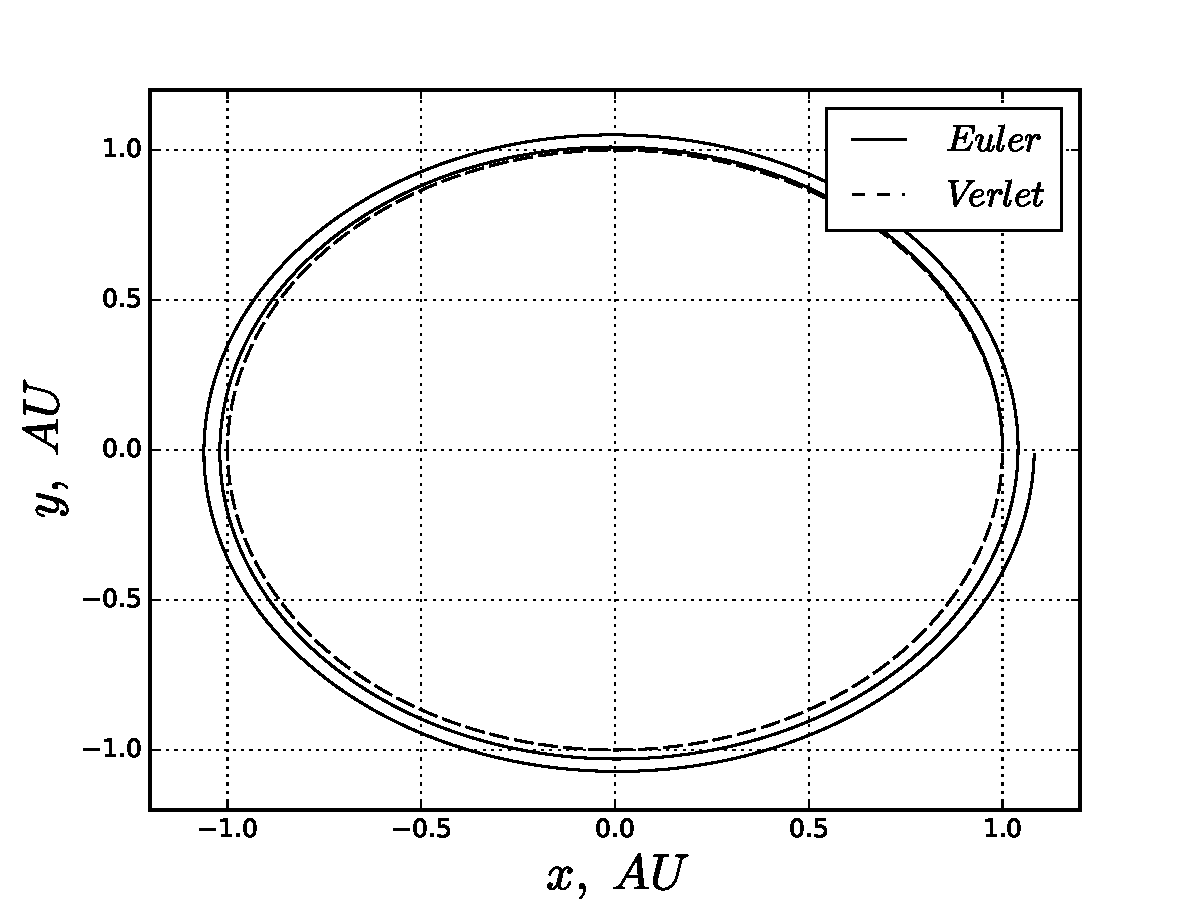
\includegraphics[scale=0.5]{eu_vs_vl}
    \caption {Orbit of the Earth around the Sun(fixed in the coordinate origin) during two earth's years. It is easy to see that Euler's method gives not stable resul. Initial velosity of the Earth is $2\pi$ $[AU/year]$. }
    \label{fig:verlet_vs_euler}
  \end{center}

\vspace*{\floatsep}

  \begin{center}
    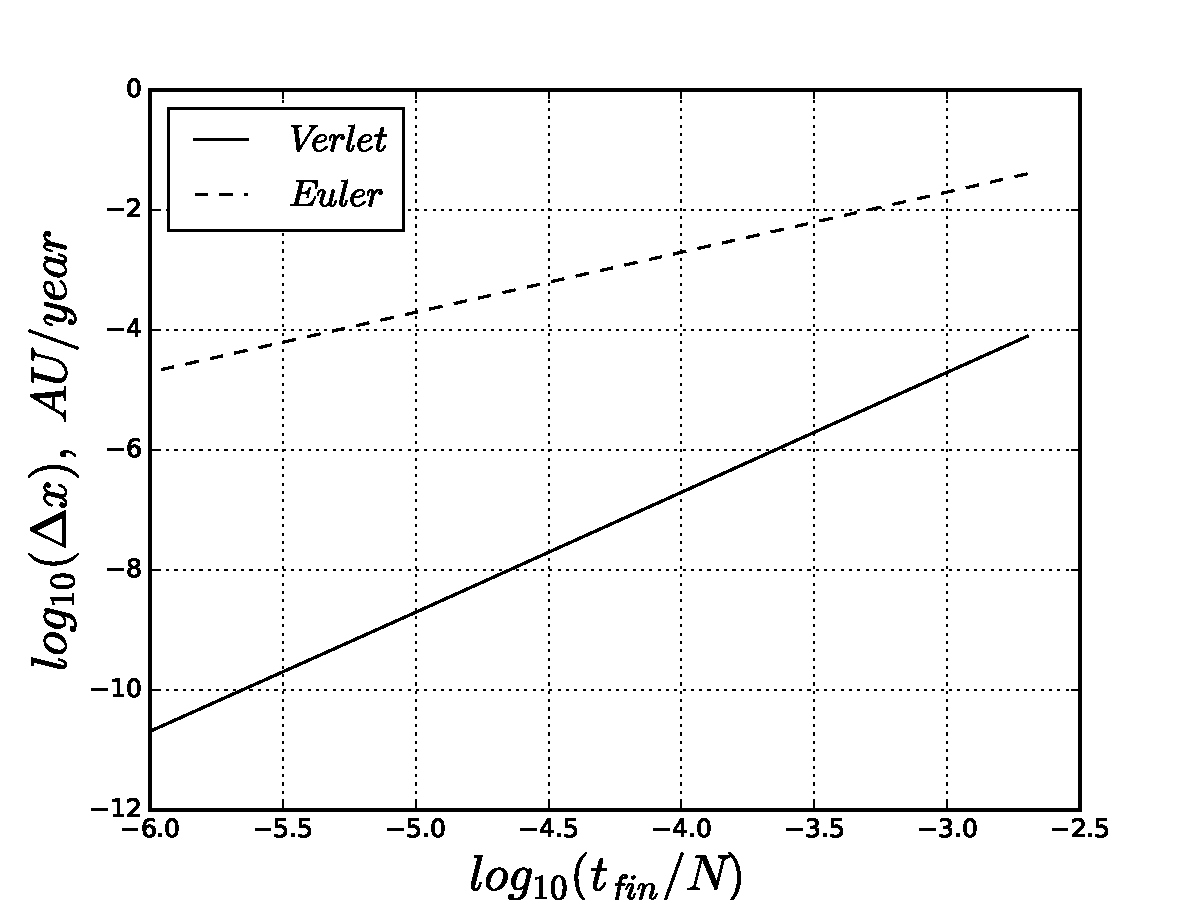
\includegraphics[scale=0.5]{c_rate}
    \caption {Convergence rate of velocity Verlet and forward Euler's methods for 2-dimensional simulation of solar system, initial velocity of the Earth is $2\pi$ $[AU/year]$, initial position of the Earth is $[1,0]\ AU$. $\Delta x$ is taken after one turn around the Sun. Range of $[500, 10^6]$ for $N$ was used in simulations. }
    \label{fig:slope}
  \end{center}
\end{figure}
\clearpage


% \begin{figure}[ht]
%   \begin{center}
%     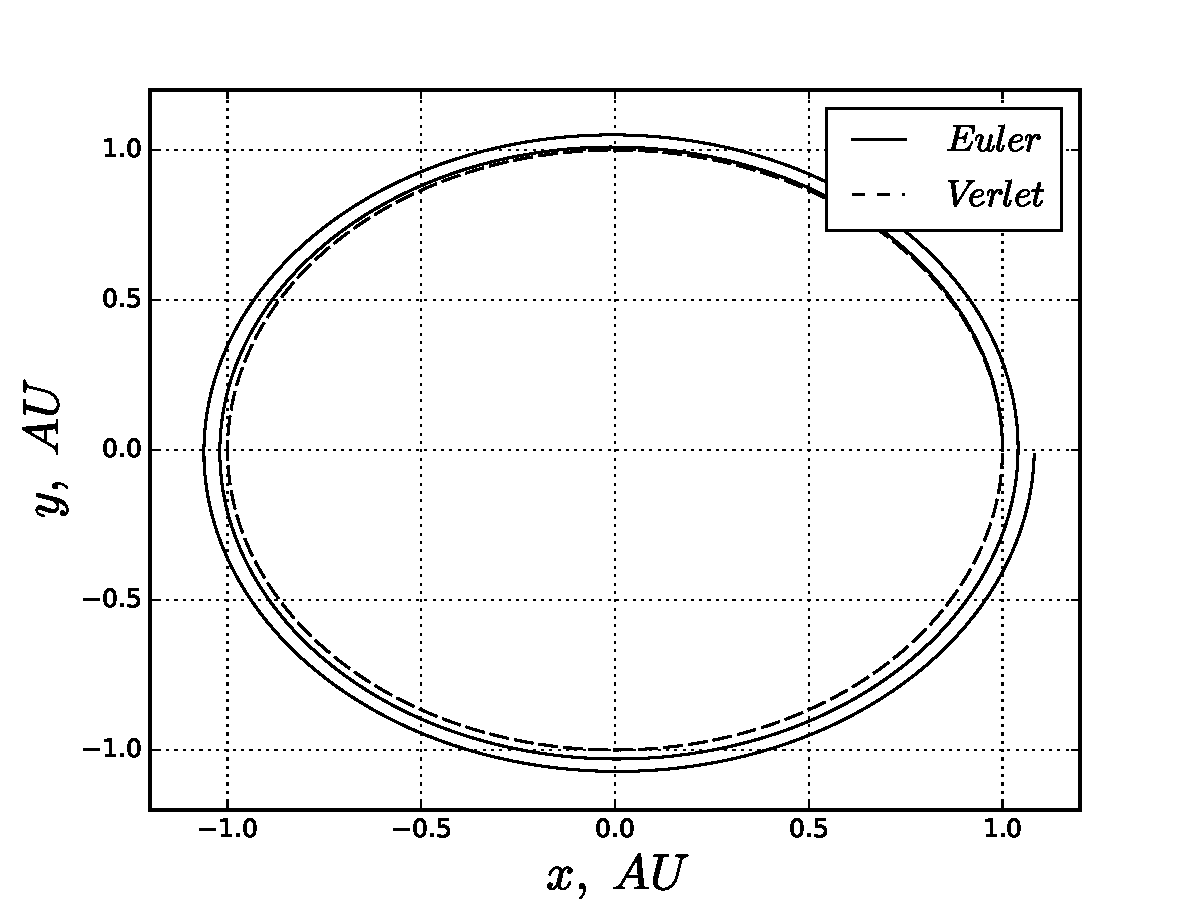
\includegraphics[scale=0.5]{eu_vs_vl}
%     \caption {Orbit of the Earth around the Sun(fixed in the coordinate origin) during two earth's years. It is easy to see that Euler's method gives not stable resul. Initial velosity of the Earth is $2\pi$ $[AU/year]$. }
%     \label{fig:verlet_vs_euler}
%   \end{center}
% \end{figure}
%
% \begin{figure}[ht]
%   \begin{center}
%     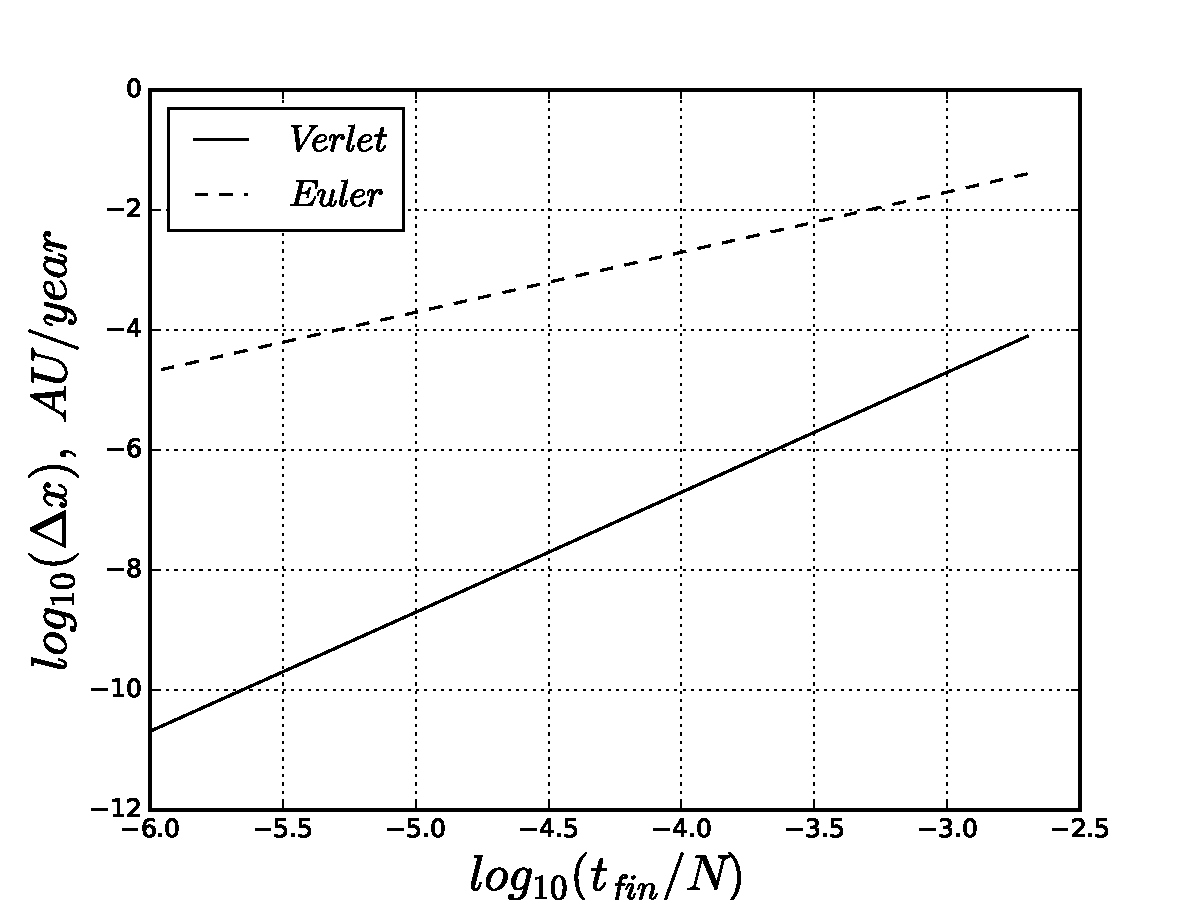
\includegraphics[scale=0.5]{c_rate}
%     \caption {Convergence rate of velocity Verlet and forward Euler's methods for 2-dimensional simulation of solar system, initial velocity of the Earth is $2\pi$ $[AU/year]$, initial position of the Earth is $[1,0]\ AU$. $\Delta x$ is taken after one turn around the Sun. Range of $[500, 10^6]$ for $N$ was used in simulations. }
%     \label{fig:slope}
%   \end{center}
% \end{figure}
\newpage
\begin{figure}[ht]
  \begin{center}
    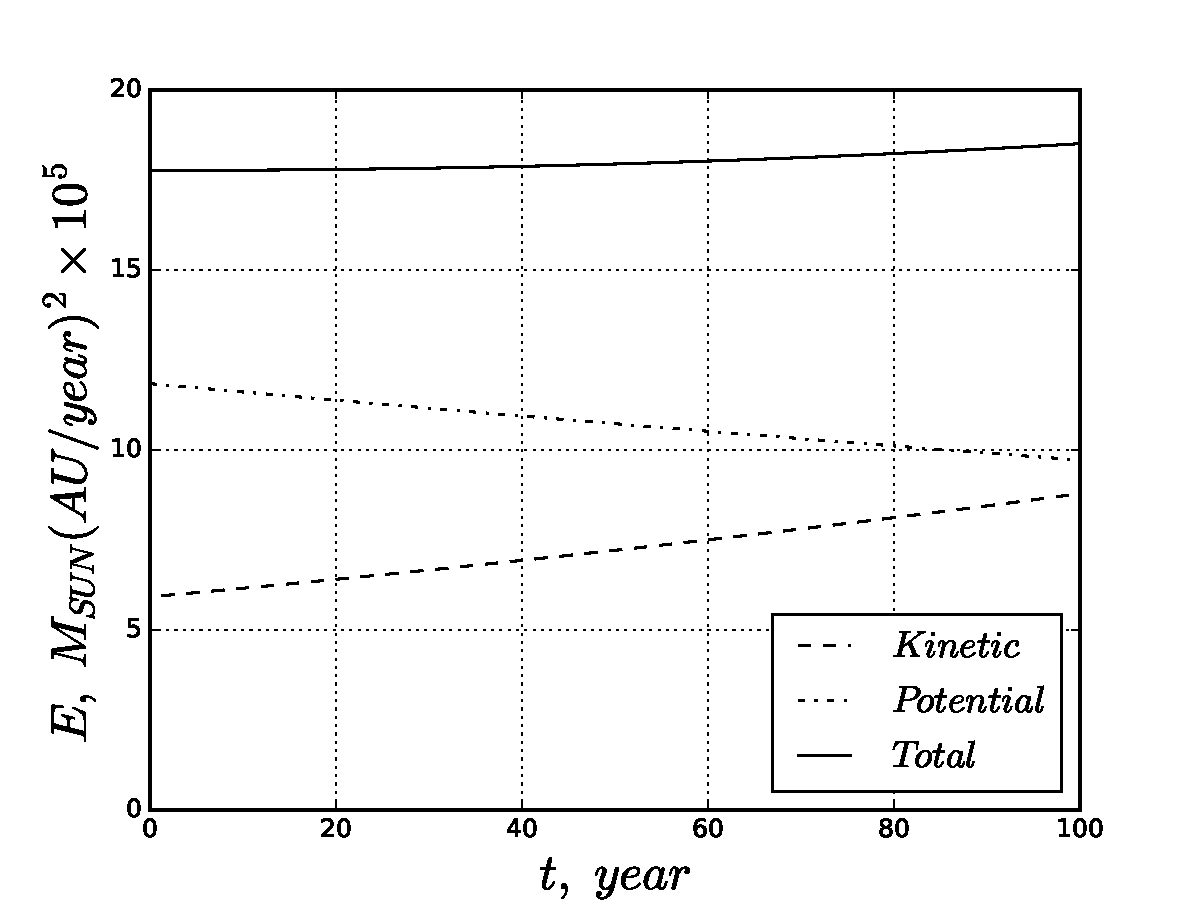
\includegraphics[scale=0.5]{euler_energy}
    \caption {Total, kinetic and potential energies for 2-dimensional simulation of solar system computed using Euler method.  Initial velocity of the Earth is $2\pi$ $[AU/year]$, initial position of the Earth is $[1,0]\ AU$. Finish time is $100$ years. $N=10^6$ was used in simulations. }
    \label{fig:euler_energy}
  \end{center}

\vspace*{\floatsep}

  \begin{center}
    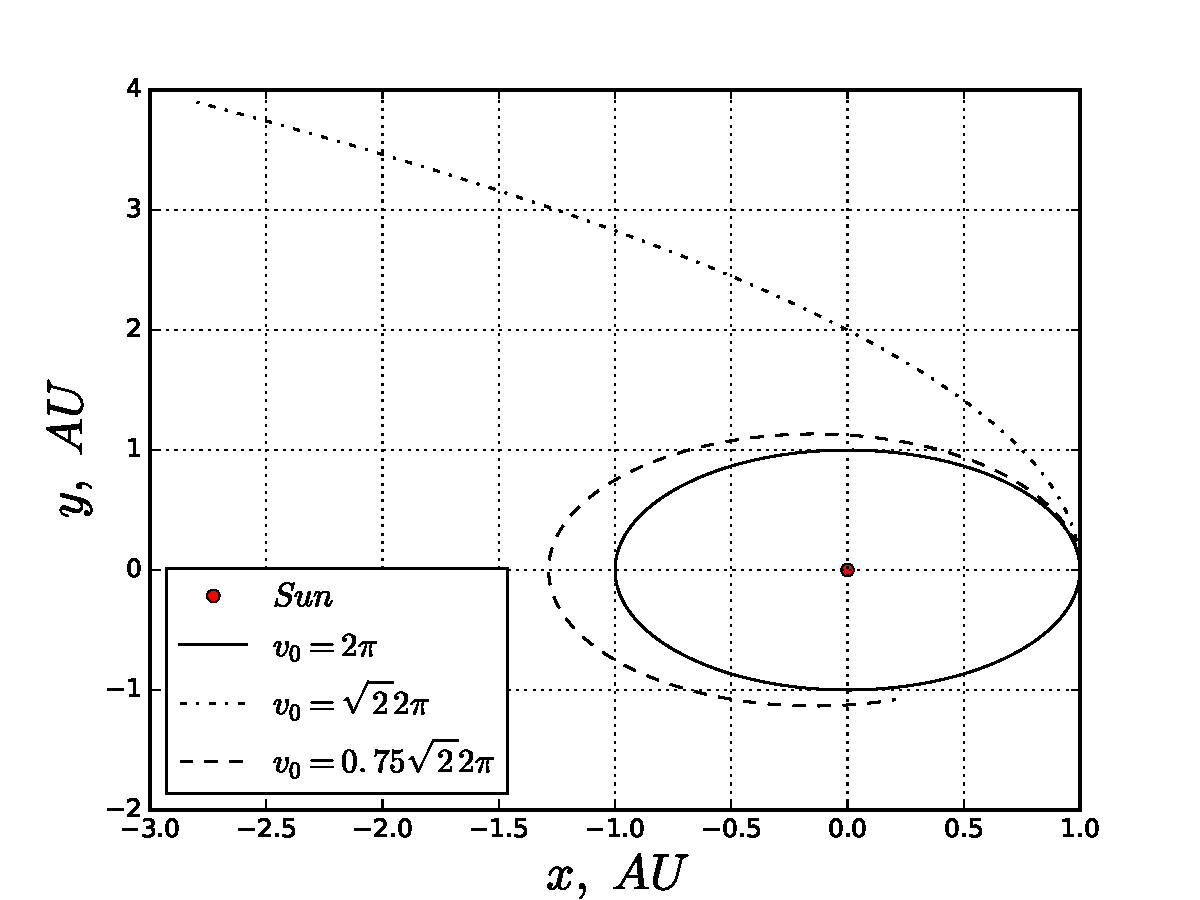
\includegraphics[scale=0.5]{escape_earth}
    \caption {Earth orbit after 2-dimensional simulation of solar system with different initial velocities of the Earth computed using velocity Verlet method. Initial position of the Earth is $[1,0]\ AU$. Finish time is $1$ years. $N=10^6$ was used in simulations. }
    \label{fig:escape}
  \end{center}
\end{figure}
\clearpage

\newpage
\subsection{Implementation and simulation}
In part \ref{Part1} we showed that for three bodies equations of motion \ref{eq:motion} transform to \ref{eq:motion-3-earth}. Number of equations grows dramatically not to mention changing number of terms in each equation. It's obvious that programming approach we used before not convenient for eight planets as we need to take into account 48 coupled ODE for eight planets in three dimensions.
If we ignore bad readability of code, difficulties in it's maintenance and debugging we may mention at least that it's very time consuming to type all equations into a code. Additionally it require a lot of boring mathematics. To avoid all mentioned difficulties we use object oriented approach of programming. In the first place we created a object oriented code and tested it on two-body system Earth-Sun. In order to test correctness of implementation we run the simulations for the Earth's initial velocity equal to so-called escape velocity. The escape velocity in this case is the required initial velocity for the Earth enough to escape the gravity of the Sun. It can be calculated by hand. We are not providing the calculations here, because they are rather trivial. This quantity appears to be a good test for our simulations. We tested the system for the two cases: for the first one we provide Earth with higher velocity then $2\pi$ $ [\frac{AU}{YEAR}]$, but not as big as the escape one and for the second case we assume the Earth has the escape velocity we have calculated manually. The result of such simulation is presented on a fig. \ref{fig:escape}. As one can see from the plot the escape velocity is equal to $\sqrt{2}2\pi $ $[\frac{AU}{YEAR}]$ and the Earth is actually escaping the system. For the velocity equal to $0.75$ of the escape velocity the orbit of the Earth is no longer circular, but it is still closed, so the Earth still cannot escape the Solar system.
After doing this we continued working with three body system. We have tested it for the most heavy planet in our Solar System, namely Jupiter. As one can see from fig. \ref{fig:3body_orig_jup} we obtain reasonable results for such simulation. Now we can play around and investigate how Jupiter influences the movement of the Earth. In order to do this we made simulations for different masses of the Jupiter, namely $10\times M_{J}$(fig. \ref{fig:3body_10x_jup}) and $1000\times M_{J}$. For the latter we got a system similar to what is called a double star. One can see it on the figure \ref{fig:3body}. This plot shows how th Earth move if we add one more star to our Solar system. The initial position and velocity for a new star as those for the Jupiter (data provided by NASA\cite{three}). The mass of a new star is 0.95 mass of the Sun. This was a heavy simulation. We took the period of 50 years and choose the time step equal to $10^{-5} [year]$. For bigger time steps the Earth escapes such Solar system immediately. For rather small time step one may see that the Earth is no longer orbiting the Sun or a new star. Such system is not stable, after 50 years the Earth actually escapes the system.
Finally we add all planets of our solar system and Pluto for historical reasons. Source code can be found \url{https://github.com/andrei-fys/fys4150/tree/master/Project_3/src/OOP/Solar_System_all_planets}. Code produces output in xyz-file format that is commonly used for molecular dynamics simulations and it's easy to visualize. We used Ovito\cite{ovito} to make a 3D visualization for our Solar system. We obtain a good model of the Solar system. It is stable over time and gives us relevant results for the escape velocity, energy and momentum conservation, etc. We also made simulations for Mercury's perihelion\ref{fig:perihelion} by general relativity correction to the Newtonian gravitational force. This time we made a simulation only for Mercury and the Sun in order to neglect the influence of other planets and calculate the pressesion caused by the general relativity effects only. We run the simulation for one century and find out that the perihelion pressesion is very close to the observed one.

\clearpage

\newpage
\begin{figure}[ht]
  \begin{center}
    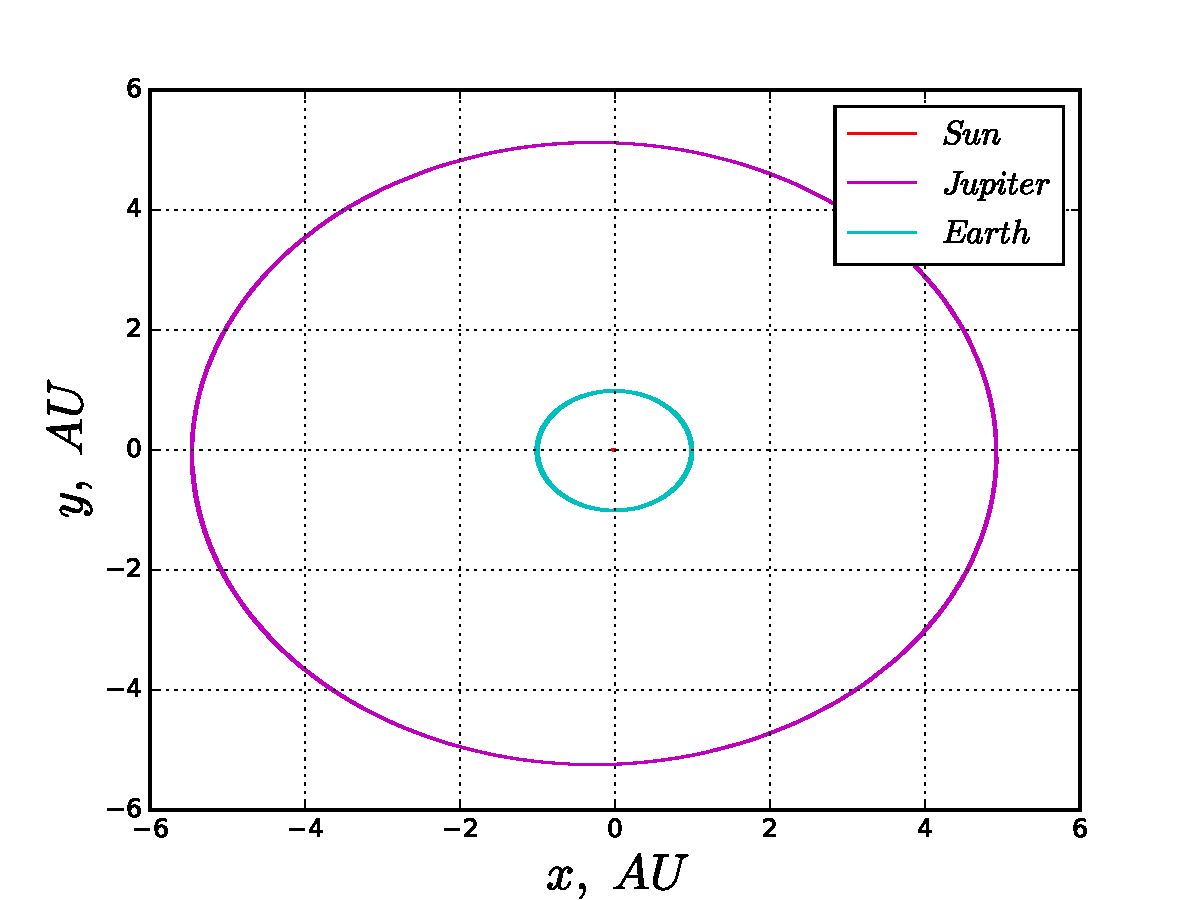
\includegraphics[scale=0.5]{3body_orig_jup}
    \caption {The simulation result for Earth and Jupiter orbiting the Sun. Time period is DOPISAT}
    \label{fig:3body_orig_jup}
  \end{center}
\vspace*{\floatsep}
  \begin{center}
    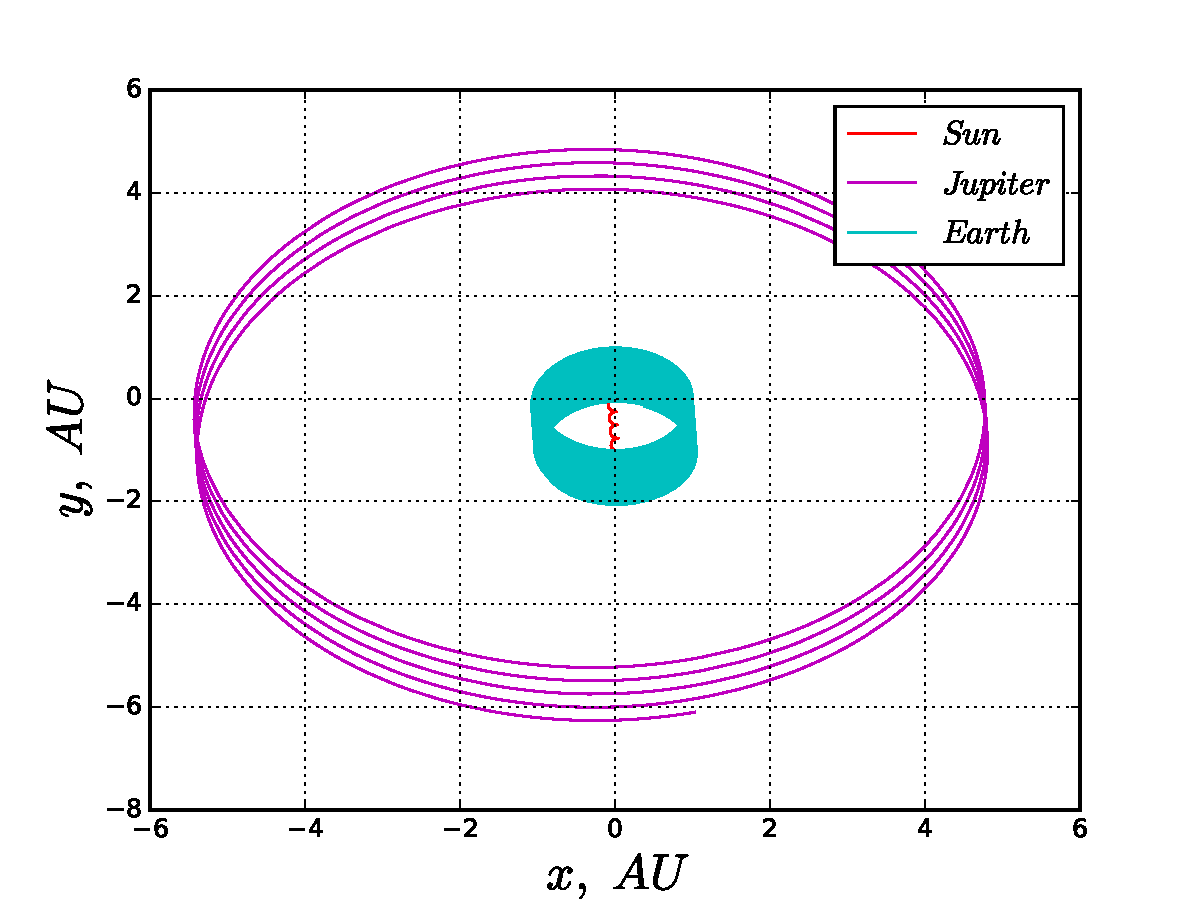
\includegraphics[scale=0.5]{3body_10x_jup}
    \caption {The simulation result for Earth and Jupiter orbiting the Sun. The mass of Jupiter is increased to by the factor of 10.}
    \label{fig:3body_10x_jup}
  \end{center}
\end{figure}
\clearpage

\newpage
\begin{figure}[ht]
  \begin{center}
    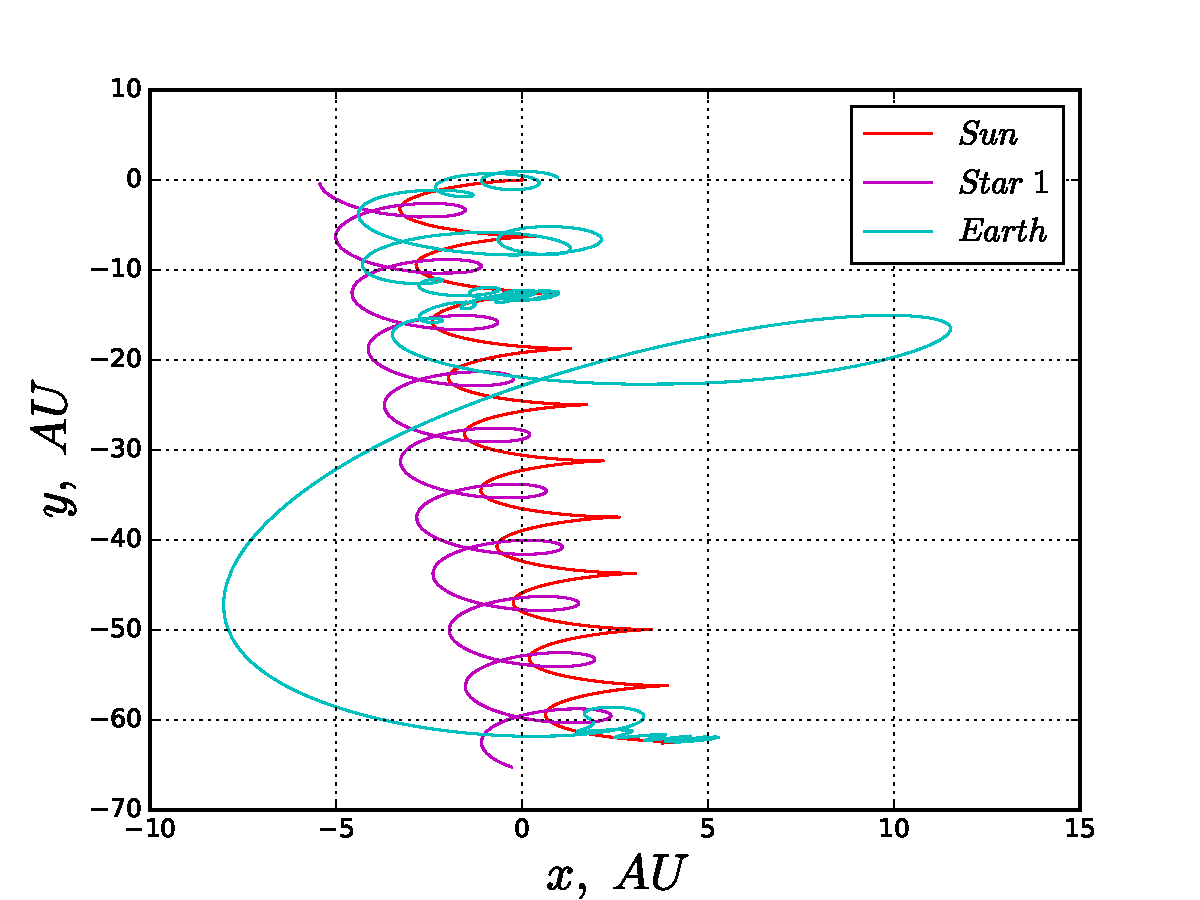
\includegraphics[scale=0.5]{3body}
    \caption {The simulation result for the Earth moving in the double star solar system. The new star has mass $0.95\times M_{Sun}$ and its initial velocity and position are those for the Jupiter.}
    \label{fig:3body}
  \end{center}

% 1 mass of the sun and 0.95 mass of the sun. dt 10⁻5, 50 years. Initial velocities from NASA 11 oct 2016, position and velocity coincide with those for Jupiter. 
  
\vspace*{\floatsep}
  \begin{center}
    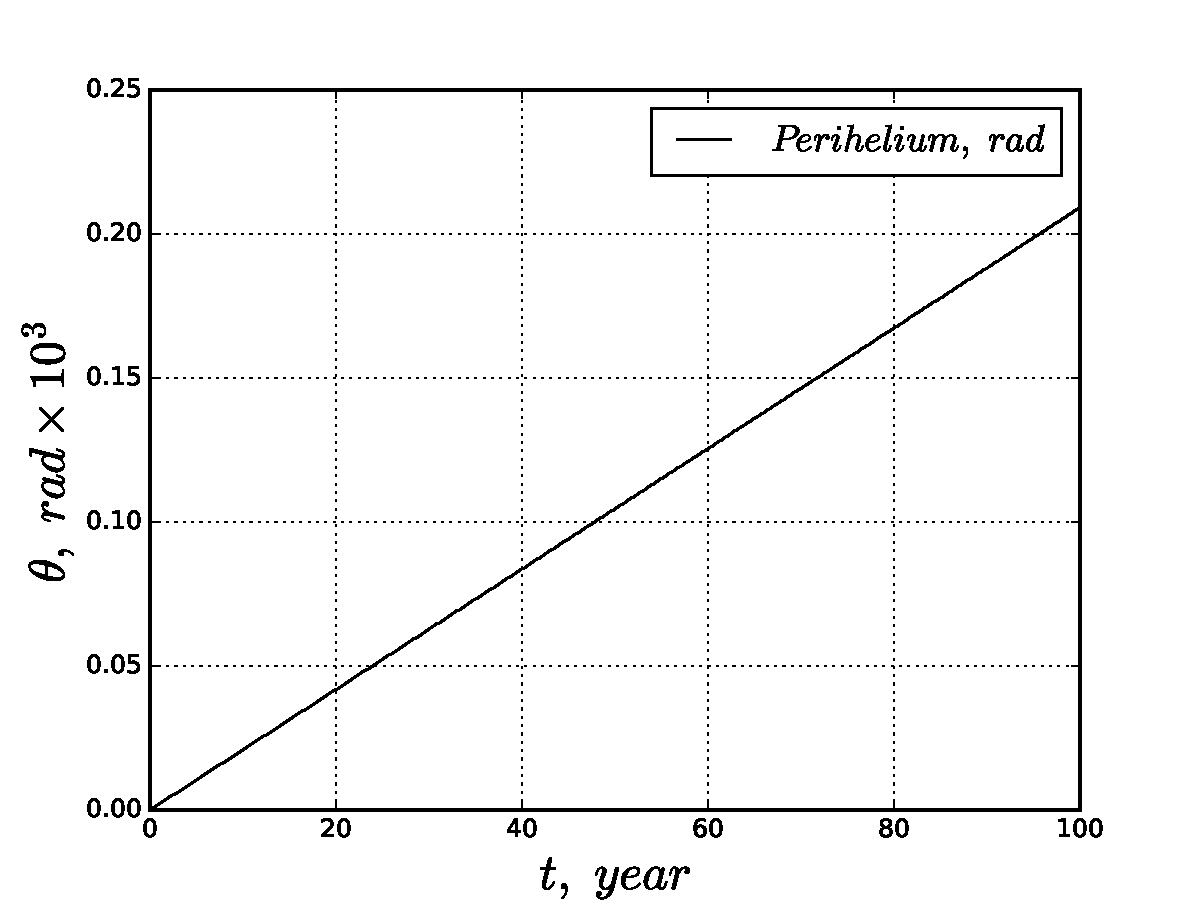
\includegraphics[scale=0.5]{mercury}
    \caption {Value of the perihelion angle obtained by simulation of Mercury’s orbit around the Sun with no other planets present. General theory of relativity precession is calculated only, classical effects are substracted. Initial position of the Mercury is $[0.3075,0]\ AU$, initial velocity is $12.44\ AU/yr$. Finish time is $100$ Earth's years. $N=10^8$ was used in simulations. }
    \label{fig:perihelion}
  \end{center}
\end{figure}
\clearpage

\newpage
\clearpage
\section{Conclusion and further research}\label{conc}
In the project we made a simulation for all planets in Solar system. Our results turn to be rather accurate and the method we chosen turn to be stable. However, we may improve this by choosing the so-called adaptive methods. The point is all planets have different periods while orbiting the Sun, so it would be nice to have more mesh points in the discretization for some of them and less for the others. This would be a nice option for futher research.For instance, one may chose some other numerical methods to solve ODE's. For example the Runge-Kutta family has may different method base on prediction correction approach (this is still the finite difference methods) and some of them provide an option to adapt the number of mesh points for different cases.
Regarding program itself there is a big potential to further development, for example adding one more class for solar system containing celestial bodies we can easily add comets and asteroid belts. Also, one may use it to model other types of Solar systems. We scratch the surface of the double star systems here, but it actually a large field for research. In 2012 the group of scientists from NASA and Tel-Aviv University in Israel discovered the double star system Kepler 47, with one of the stars very similar to our Sun \cite{kepler}. By some small corrections our program can by modified to simulate this system. We consider systems of double stars rather interesting topic and actually planned to discuss it more in the project, but have to give up the idea due to the lack of time.


\clearpage
\newpage
\begin{thebibliography}{2}
\bibitem{one} 
Morten Hjorth-Jensen. 
\textit{Computational Physics
}. 
Lecture Notes Fall 2015, August 2015.

\bibitem{two} 
W. Press, B. Flannery, S. Teukolsky, W. Vetterling. 
\textit{Numerical Recipes in C++, The art of scientific Computing}. 
Cambridge University Press, 1999.

\bibitem {three}
NASA.
\url{http://ssd.jpl.nasa.gov/horizons.cgi#top}.


\bibitem {ovito}
A. Stukowski.
\textit{
Visualization and analysis of atomistic simulation data with OVITO - the Open Visualization Tool
Modelling Simul. Mater. Sci. Eng. 18 (2010), 015012}
Phys. Rev. A 57, 120 – Published 1 January 1998.

\bibitem {kepler}
Orosz, Jerome A. and others.
\textit
{"Kepler-47: A Transiting Circumbinary Multiplanet System". 
}
Science. vol. 337, num. 6101, pp. 1511--1514, 2012. 
 
\end{thebibliography}

\end{document}
